\section{Model Verification}
\label{sec:model_verification}
In order to confidently use the model developed in the modelling chapter~\vref{ch:modelling}, it is important to verify that it actually reflect the real behaviour of the ship. This section will be used as a sanity check for the model and give indication of how well the model fits with the real ship.

As the hydrodynamic model parameters has been determined in the appendix\vref{app:damping}, using the state space representation presented in \vref{eq:ss}, it can be used to verify the complete simulation model.

\subsection{Step Response}
A step response of the model can be used to verify the steady state input-output relations. This can both give the steady state but also the time constant to verify the system. This can be done by accelerating the vessel from steady state and measure the velocity curve of the ship. The vessel will reach zero acceleration witch implies constant velocity, from where the time constant can be measured. This time constant needs to be approximately the same for the vessel and the model of the vessel. All the steady state input-output relations will be approximately the same, i.e. like the time constant in surge. The same kind of test may be performed from all steady state scenarios, but the critical is the surge velocity, that ensures that the vessel reaches the correct velocity and decelerates again. The model have been tested in surge, which can be seen on figure \ref{fig:surgevel}. On the figure can be seen that the vessel accelerates to a constant surge velocity, which is also assumed to happen. Afterwards, when then input it set to zero, the velocity will go toward zero and the vessel will be still in position. On the lower half of the figure is the pitch angle represented. This pitch does not apply the assumptions and observations from the real AAUSHIP. It can be noted that the pitch angle is very small, being $\theta = 6\cdot 10^{-3}\ $rad. This corresponds to a pitch angle of $\theta = 0.34\arcdeg$. This is not a correct value of the pitching angle, but the work with the model does not seem to uncover why this angle is not correct. It is expected by observation that the pitch angle should be around $\approx 4 \arcdeg$ which is far from what the model predicts. Though after trying to locate the error, it is assessed that this is not that critical an error. This is due to the fact it does not have an influence of how the model will perform while surging. The correct pitch angle can be read from the sensors and used to make the post processing of the seabed data from the surveying.

\begin{figure}
  \centering
  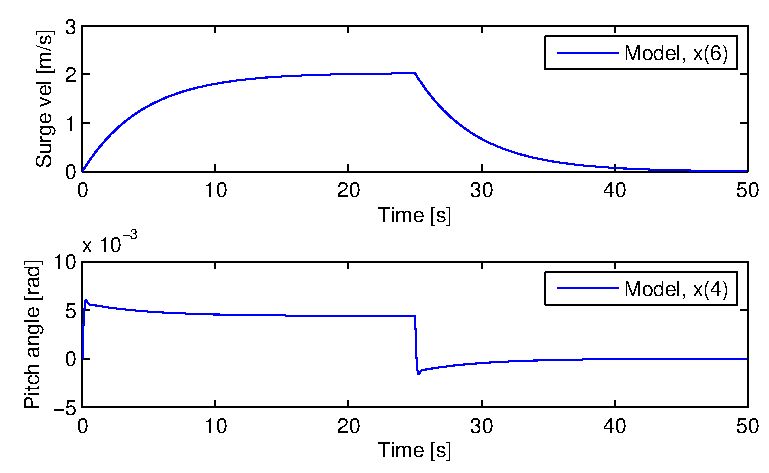
\includegraphics[width=0.8\textwidth]{../../code/matlab/surgemodel}
  \caption{The output of the model in surge, where constant input is applied and after some time set to zero.}
  \label{fig:surgevel}
\end{figure}

\subsection{Stability}
A stability analysis can be conducted by examining the eigenvalues of the system. To ensure stability it is a criteria that the eigenvalues should all be stable for this system. This is fulfilled if the real part of all the eigenvalues of the system are negative, which implies a stable fixed point.

Stability of the discretised version also has to be checked by ensuring that the pole-zero map is within the unit circle. The eigenvalues of the Jacobian also needs to have absolute value less than one, which implies placement within the unit circle. If these are placed within the unit circle it is also a fixed point. If just one eigenvalue is greater than one it implies instability. If the eigenvalue is exactly equal to one it needs further investigation by looking more into the Jacobian.

\subsection{Simulation of the Model}
A final verification is to compare the correlation between a sea trail operated by human operator. It is desired to make manoeuvres similar to what the system is supposed to perform with focus on the surge velocity. That is i.e. making a test with the same input as given to the model in figure \ref{fig:surgevel}. The velocities should map approximately with each other within an acceptable level. Four tests with the same input as in figure \ref{fig:surgevel} have been showed on figure \ref{fig:surgeverify}.

\begin{figure}
  \centering
  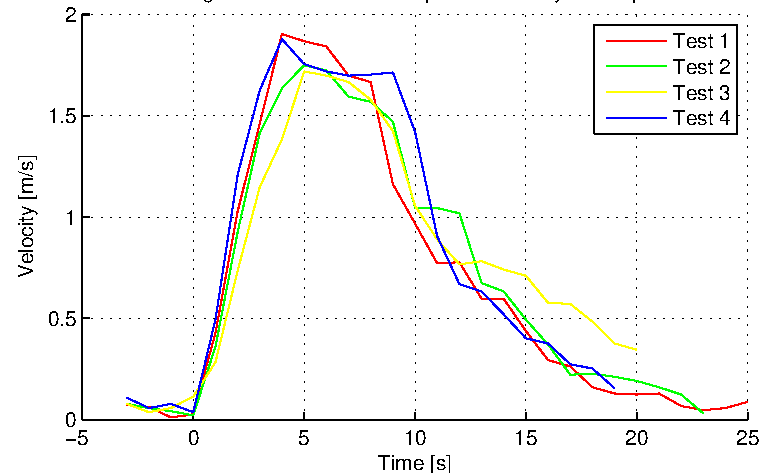
\includegraphics[width=0.8\textwidth]{../../code/matlab/log-viewer/surgeverify}
  \caption{Surge tests with constant input followed by zero input.}
  \label{fig:surgeverify}
\end{figure}

The comparison between those shows that the constant surge velocity is approximately the same. The measurements is a little lower in the velocity but not at a critical level. The damping of the system has been determined from appendix \ref{app:damping}, thus is the damping also a relatively good match. In both cases, the model and the measurements, it takes about 20s for the vessel to reach almost zero velocity. Though since the model is linear it does not cover the extreme input to the system, thus is the measurement at the accelerating ramp much faster than the model predicts it to be. Since the vessel is assumed to reach and sail with constant velocity is this problem not as critical as it seems.
The pitch angle are as concluded above not correct. To verify that the form of the pitch angle are correct has the measurements from the surge tests been compared with the pitch angles. The results of the pitch angle for a surge test can be seen on figure \ref{fig:pitchverify}.

\begin{figure}
  \centering
  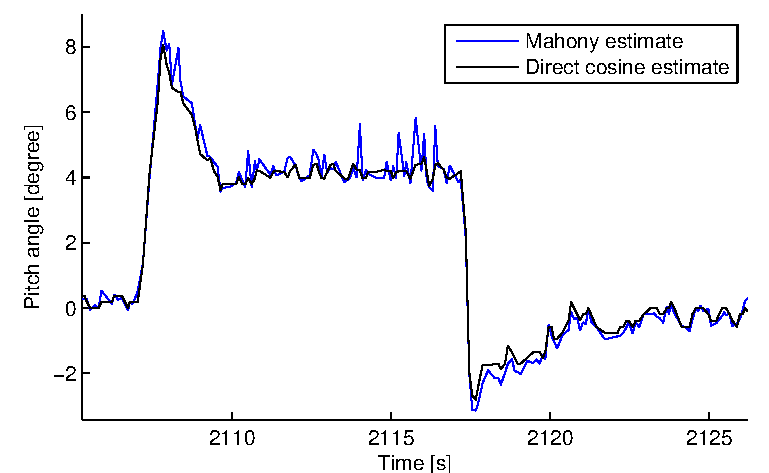
\includegraphics[width=0.8\textwidth]{../../code/matlab/log-viewer/pitchverify}
  \caption{Surge tests with constant input followed by zero input.}
  \label{fig:pitchverify}
\end{figure}

The pitch angle is rising above the steady state of the constant velocity, since the forward thrust is as high as it is. Then the vessel tilts a little down and reaches a steady angle at $\approx 4\arcdeg$, which is also as observed during testing. When the input is set to zero the vessel will decelerate and the pitch will become a little negative around zero due to the high damping factor, and then settle at new steady state, determined by the physics of the vessel and the restoring forces. The value of the pitching angles are as expected from the observations, even though the model does not evaluate the correct pitching angle.